\documentclass[12pt,a4paper]{article}

% 导入必要的宏包
\usepackage[UTF8]{ctex}
\usepackage{geometry}
\usepackage{amsmath}
\usepackage{amsfonts}
\usepackage{amssymb}
\usepackage{graphicx}
\usepackage{enumitem}
\usepackage{xcolor}
\usepackage{tikz}
\usepackage{float}
\usepackage{hyperref}
\usepackage{multicol}
\usepackage{longtable}
\usepackage{array}
\usepackage{tabularx}
\usepackage{listings}

% 代码高亮设置
\lstset{
    basicstyle=\ttfamily\small,
    keywordstyle=\color{blue},
    commentstyle=\color{green!70!black},
    stringstyle=\color{red},
    breaklines=true,
    numbers=left,
    numberstyle=\tiny\color{gray},
}

% 页面设置
\geometry{left=2.5cm,right=2.5cm,top=2.5cm,bottom=2.5cm}

% 标题页设置
\title{\textbf{2022年数据结构题库} \\ \large 单项选择题与综合应用题详解}
\author{}
\date{}

% 定义题型环境
\newenvironment{choicequestion}[1][]{%
    \vspace{0.5cm}
    \noindent\textbf{[#1]}
    \vspace{0.2cm}
}{}

\newenvironment{answersection}{%
    \vspace{0.2cm}
    \noindent\textbf{[参考答案]}\\
    \vspace{0.1cm}
}{}

\newenvironment{analysissection}{%
    \vspace{0.2cm}
    \noindent\textbf{[答案解析]}\\
    \vspace{0.1cm}
}{}

% 定义题号计数器
\newcounter{questioncounter}

% 定义题号计数器
\newcounter{questioncounter}

% 问题格式化命令
\newcommand{\question}[2]{%
    \stepcounter{questioncounter}%
    \noindent\textbf{\thequestioncounter} #1%
}

% 选择题选项格式
\newcommand{\choices}[4]{%
    \begin{multicols}
    \noindent \textbf{A.} #1 \par
    \noindent \textbf{B.} #2 \par
    \noindent \textbf{C.} #3 \par
    \noindent \textbf{D.} #4 \par
    \end{multicols}%
}

% 开始文档
\begin{document}

\maketitle

\section{单项选择题}

\begin{choicequestion}[单选题]
\question{下列程序段的时间复杂度是（ ）。\newline
\begin{lstlisting}[language=C]
int sum = 0;  
for (int i = 1; i < n; i *= 2)  
    for (int j = 0; j < i; j++)  
        sum++;
\end{lstlisting}}{}

\choices{$O(\log n)$}{O(n)}{$O(n \log n)$}{$O\left(n^{2}\right)$}

\begin{answersection}
B. O(n)
\end{answersection}

\begin{analysissection}
外层循环中 $i$ 的取值为 $1,2,4,8,\dots,2^k$（其中 $2^k < n$），共执行 $\lfloor \log_2 n \rfloor$ 次。内层循环执行次数分别为 $1,2,4,\dots,2^k$。总执行次数为 $1+2+4+\dots+2^k = 2^{k+1}-1 < 2n$，因此时间复杂度为 $O(n)$。
\end{analysissection}
\end{choicequestion}

\begin{choicequestion}[单选题]
\question{给定有限符号集 S, in 和 out 均为 S 中所有元素的任意排列。对于初始为空的栈 ST, 下列叙述中, 正确的是 ( )。}{}

\choices{若 in 是 ST 的入栈序列, 则不能判断 out 是否为其可能的出栈序列}{若 out 是 ST 的出栈序列, 则不能判断 in 是否为其可能的入栈序列}{若 in 是 ST 的入栈序列, out 是对应 in 的出栈序列, 则 in 与 out 一定不同}{若 in 是 ST 的入栈序列, out 是对应 in 的出栈序列, 则 in 与 out 可能互为倒序}

\begin{answersection}
D. 若 in 是 ST 的入栈序列, out 是对应 in 的出栈序列, 则 in 与 out 可能互为倒序
\end{answersection}

\begin{analysissection}
当所有元素依次入栈后，再依次出栈时，出栈序列（out）恰好是入栈序列（in）的逆序。这是栈“后进先出”特性的直接体现。
\end{analysissection}
\end{choicequestion}

\begin{choicequestion}[单选题]
\question{若结点 $\mathfrak{p}$ 与 $\mathbf{q}$ 在二叉树T的中序遍历序列中相邻，且 $\mathfrak{p}$ 在 $\mathbf{q}$ 之前，则下列 $\mathfrak{p}$ 与 $\mathbf{q}$ 的关系中，不可能的是（）。\newline
I. q是p的双亲\newline
II. $\mathbf{q}$ 是 $\mathfrak{p}$ 的右孩子\newline
III. q是p的右兄弟\newline
IV. q是p的双亲的双亲}{}

\choices{仅 I}{仅 III}{仅 II、III}{仅 II、IV}

\begin{answersection}
C. 仅 II、III
\end{answersection}

\begin{analysissection}
中序遍历序列为“左子树—根—右子树”。p在q之前且二者相邻：

- I 可能：q是p的双亲，且p是q的左子树中最右结点；
- II 不可能：若q是p的右孩子，则p之后应先遍历p的右子树（至少包含q），不可能p与q直接相邻；
- III 不可能：若q是p的右兄弟，则p与q之间至少存在其共同双亲结点，不可能相邻；
- IV 可能：q是p的双亲的双亲（祖父），p是左子树中最右结点时可满足相邻。

故不可能的是II和III。
\end{analysissection}
\end{choicequestion}

\begin{choicequestion}[单选题]
\question{若三叉树 T 中有 244 个结点（叶结点的高度为 1），则 T 的高度至少是（）。}{}

\choices{8}{7}{6}{5}

\begin{answersection}
C. 6
\end{answersection}

\begin{analysissection}
要使高度最小，树应尽可能充满。满三叉树（每层节点数为 $3^{h-1}$）的高度为h时，结点总数为 $\frac{3^h - 1}{2}$。

- 高度5：$\frac{3^5 - 1}{2} = 121$；
- 高度6：$\frac{3^6 - 1}{2} = 364$。

由于 $121 < 244 < 364$，故T的高度至少为6。
\end{analysissection}
\end{choicequestion}

\begin{choicequestion}[单选题]
\question{对任意给定的含 $n$ （ $n > 2$ ）个字符的有限集 S，用二叉树表示 S 的哈夫曼编码集和定长编码集，分别得到二叉树 T1 和 T2。下列叙述中，正确的是（）。}{}

\choices{T1 与 T2 的结点数相同}{T1 的高度大于 T2 的高度}{出现频次不同的字符在 T1 中处于不同的层}{出现频次不同的字符在 T2 中处于相同的层}

\begin{answersection}
C. 出现频次不同的字符在 T1 中处于不同的层
\end{answersection}

\begin{analysissection}
哈夫曼树（T1）中，字符的编码长度由其出现频次决定，频次越低，编码越长，所在层数通常越高（不同频次的字符一般处于不同层）。定长编码树（T2）中所有字符编码长度相同，叶子结点处于同一层或相邻两层。
\end{analysissection}
\end{choicequestion}

\begin{choicequestion}[单选题]
\question{对于无向图 $\mathbf{G} = (\mathrm{V},\mathrm{E})$ ，下列选项中，正确的是（ ）。}{}

\choices{当 $|\mathrm{V}| > |\mathrm{E}|$ 时， $\mathbf{G}$ 一定是连通的}{当 $|\mathrm{V}| < |\mathrm{E}|$ 时, $\mathrm{G}$ 一定是连通的}{当 $|\mathrm{V}| = |\mathrm{E}| - 1$ 时，G一定是不连通的}{当 $|\mathrm{V}| > |\mathrm{E}| + 1$ 时, $\mathrm{G}$ 一定是不连通的}

\begin{answersection}
D. 当 $|\mathrm{V}| > |\mathrm{E}| + 1$ 时, $\mathrm{G}$ 一定是不连通的
\end{answersection}

\begin{analysissection}
连通无向图至少需要 $|V|-1$ 条边（形成一棵生成树）。当 $|E| < |V|-1$，即 $|V| > |E| + 1$ 时，图中必然存在孤立部分，故一定不连通。
\end{analysissection}
\end{choicequestion}

\begin{choicequestion}[单选题]
\question{在下图所示的5阶B树T中，删除关键字260之后需要进行必要的调整，得到新的B树T1。下列选项中，不可能是T1根结点中关键字序列的是（）。}{}

\begin{figure}[H]
\centering
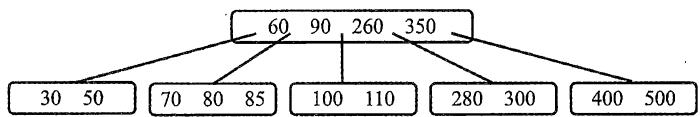
\includegraphics[width=0.3\textwidth]{images/c959dbeb0f460d2b6a52a2c8773b071073085434664b3fe53f5fd85c9477ea13.jpg}
\end{figure}

\choices{60, 90, 280}{60, 90, 350}{60, 85, 110, 350}{60, 90, 110, 350}

\begin{answersection}
C. 60, 85, 110, 350
\end{answersection}

\begin{analysissection}
5阶B树每个结点最多容纳4个关键字。删除260后，根据B树删除规则（借位或合并），根结点关键字序列必须保持有序且满足结点关键字数限制。选项C中出现了85，而原树中260所在结点的调整无法产生该序列，故不可能。
\end{analysissection}
\end{choicequestion}

\begin{choicequestion}[单选题]
\question{下列因素中，影响散列（哈希）方法平均查找长度的是（ ）。\newline
I. 装填因子\newline
II. 散列函数\newline
III. 冲突解决策略}{}

\choices{仅 I、II}{仅 I、III}{仅 II、III}{I、II、III}

\begin{answersection}
D. I、II、III
\end{answersection}

\begin{analysissection}
装填因子影响冲突发生的概率；散列函数的均匀性影响冲突分布；冲突解决策略（线性探测、链地址等）直接决定查找时的比较次数。三者均会影响平均查找长度。
\end{analysissection}
\end{choicequestion}

\begin{choicequestion}[单选题]
\question{使用二路归并排序对含 $n$ 个元素的数组 M 进行排序时，二路归并操作的功能是（）。}{}

\choices{将两个有序表合并为一个新的有序表}{将 M 划分为两部分, 两部分的元素个数大致相等}{将 $\mathbf{M}$ 划分为 $n$ 个部分, 每个部分中仅含有一个元素}{将 M 划分为两部分, 一部分元素的值均小于另一部分元素的值}

\begin{answersection}
A. 将两个有序表合并为一个新的有序表
\end{answersection}

\begin{analysissection}
二路归并排序的核心步骤是将两个已排好序的子序列合并成一个有序序列。
\end{analysissection}
\end{choicequestion}

\begin{choicequestion}[单选题]
\question{对数据进行排序时，若采用直接插入排序而不采用快速排序，则可能的原因是（）。\newline
I. 大部分元素已有序\newline
II. 待排序元素数量很少\newline
III. 要求空间复杂度为 $O(1)$\newline
IV. 要求排序算法是稳定的}{}

\choices{仅 I、II}{仅 III、IV}{仅 I、II、IV}{I、II、III、IV}

\begin{answersection}
D. I、II、III、IV
\end{answersection}

\begin{analysissection}
- I：数据基本有序时，插入排序接近 $O(n)$，优于快速排序；
- II：数据量小时，插入排序常数小、更高效；
- III：插入排序空间复杂度 $O(1)$，而快速排序平均需要 $O(\log n)$ 栈空间；
- IV：插入排序是稳定排序，快速排序不稳定。

四条原因均成立。
\end{analysissection}
\end{choicequestion}

\section{综合应用题}

\begin{choicequestion}[问答题]
\question{(13分)已知非空二叉树T的结点值均为正整数，采用顺序存储方式保存，数据结构定义如下：\newline

\begin{lstlisting}[language=C]
typedef struct{ //MAX_SIZE为已定义常量
    int SqBiTreeNode[MAX_SIZE]; //保存二叉树结点值的数组
    int ElemNum; //实际占用的数组元素个数
}SqBiTree;
\end{lstlisting}\newline

T中不存在的结点在数组SqBiTNode中用-1表示。请设计一个尽可能高效的算法，判定一棵采用这种方式存储的二叉树是否为二叉搜索树，若是，则返回 true，否则，返回 false。要求：\newline
1）给出算法的基本设计思想。  \newline
2）根据设计思想，采用C或 $\mathrm{C}++$ 语言描述算法，关键之处给出注释。}{}

\begin{answersection}
1）算法的基本设计思想：采用递归方式，对每个结点设置取值范围（下界、上界）。根结点范围为 $(-\infty, +\infty)$；左子树结点值必须小于父结点值，右子树结点值必须大于父结点值。若所有结点均满足范围约束，则为二叉搜索树。
\end{answersection}

\begin{analysissection}
2）算法实现（C语言）：
\begin{lstlisting}[language=C]
#include <limits.h>

bool isBSTUtil(SqBiTree tree, int index, int minVal, int maxVal) {
    if (index >= tree.ElemNum || tree.SqBiTreeNode[index] == -1) {
        return true;                    // 空结点合法
    }
    
    int val = tree.SqBiTreeNode[index];
    if (val <= minVal || val >= maxVal) {
        return false;                   // 违反BST性质
    }
    
    // 递归检查左子树（上限为当前值）和右子树（下限为当前值）
    return isBSTUtil(tree, 2 * index + 1, minVal, val) &&
           isBSTUtil(tree, 2 * index + 2, val, maxVal);
}

bool isBinarySearchTree(SqBiTree tree) {
    if (tree.ElemNum == 0) return true;
    return isBSTUtil(tree, 0, INT_MIN, INT_MAX);
}
\end{lstlisting}
\end{analysissection}
\end{choicequestion}

\begin{choicequestion}[问答题]
\question{(10分)现有 $n(n > 100000)$ 个数保存在一维数组M中，需要查找M中最小的10个数。请回答下列问题。\newline
1）设计一个完成上述查找任务的算法，要求平均情况下的比较次数尽可能少，简述其算法思想（不需要程序实现）。  \newline
2）说明你所设计的算法平均情况下的时间复杂度和空间复杂度。}{}

\begin{answersection}
1）算法思想：维护一个大小为10的最大堆（优先队列）。遍历数组M：
- 若堆中元素不足10个，直接插入当前元素；
- 若当前元素小于堆顶元素，则删除堆顶元素并插入当前元素；
- 否则忽略当前元素。
遍历结束后，堆中保存的即为最小的10个数。
\end{answersection}

\begin{analysissection}
2）时间复杂度：$O(n \log 10) = O(n)$（每次堆操作复杂度为 $O(\log 10)$，共 $n$ 次操作）。\\
空间复杂度：$O(1)$（堆大小固定为常数10，与$n$无关）。
\end{analysissection}
\end{choicequestion}

\end{document}